\documentclass{article}\usepackage[]{graphicx}\usepackage[]{xcolor}
% maxwidth is the original width if it is less than linewidth
% otherwise use linewidth (to make sure the graphics do not exceed the margin)
\makeatletter
\def\maxwidth{ %
  \ifdim\Gin@nat@width>\linewidth
    \linewidth
  \else
    \Gin@nat@width
  \fi
}
\makeatother

\definecolor{fgcolor}{rgb}{0.345, 0.345, 0.345}
\newcommand{\hlnum}[1]{\textcolor[rgb]{0.686,0.059,0.569}{#1}}%
\newcommand{\hlsng}[1]{\textcolor[rgb]{0.192,0.494,0.8}{#1}}%
\newcommand{\hlcom}[1]{\textcolor[rgb]{0.678,0.584,0.686}{\textit{#1}}}%
\newcommand{\hlopt}[1]{\textcolor[rgb]{0,0,0}{#1}}%
\newcommand{\hldef}[1]{\textcolor[rgb]{0.345,0.345,0.345}{#1}}%
\newcommand{\hlkwa}[1]{\textcolor[rgb]{0.161,0.373,0.58}{\textbf{#1}}}%
\newcommand{\hlkwb}[1]{\textcolor[rgb]{0.69,0.353,0.396}{#1}}%
\newcommand{\hlkwc}[1]{\textcolor[rgb]{0.333,0.667,0.333}{#1}}%
\newcommand{\hlkwd}[1]{\textcolor[rgb]{0.737,0.353,0.396}{\textbf{#1}}}%
\let\hlipl\hlkwb

\usepackage{framed}
\makeatletter
\newenvironment{kframe}{%
 \def\at@end@of@kframe{}%
 \ifinner\ifhmode%
  \def\at@end@of@kframe{\end{minipage}}%
  \begin{minipage}{\columnwidth}%
 \fi\fi%
 \def\FrameCommand##1{\hskip\@totalleftmargin \hskip-\fboxsep
 \colorbox{shadecolor}{##1}\hskip-\fboxsep
     % There is no \\@totalrightmargin, so:
     \hskip-\linewidth \hskip-\@totalleftmargin \hskip\columnwidth}%
 \MakeFramed {\advance\hsize-\width
   \@totalleftmargin\z@ \linewidth\hsize
   \@setminipage}}%
 {\par\unskip\endMakeFramed%
 \at@end@of@kframe}
\makeatother

\definecolor{shadecolor}{rgb}{.97, .97, .97}
\definecolor{messagecolor}{rgb}{0, 0, 0}
\definecolor{warningcolor}{rgb}{1, 0, 1}
\definecolor{errorcolor}{rgb}{1, 0, 0}
\newenvironment{knitrout}{}{} % an empty environment to be redefined in TeX

\usepackage{alltt}
\usepackage{amsmath} %This allows me to use the align functionality.
                     %If you find yourself trying to replicate
                     %something you found online, ensure you're
                     %loading the necessary packages!
\usepackage{amsfonts}%Math font
\usepackage{graphicx}%For including graphics
\usepackage{hyperref}%For Hyperlinks
\usepackage[shortlabels]{enumitem}% For enumerated lists with labels specified
                                  % We had to run tlmgr_install("enumitem") in R
\hypersetup{colorlinks = true,citecolor=black} %set citations to have black (not green) color
\usepackage{natbib}        %For the bibliography
\setlength{\bibsep}{0pt plus 0.3ex}
\bibliographystyle{apalike}%For the bibliography
\usepackage[margin=0.50in]{geometry}
\usepackage{float}
\usepackage{multicol}

%fix for figures
\usepackage{caption}
\newenvironment{Figure}
  {\par\medskip\noindent\minipage{\linewidth}}
  {\endminipage\par\medskip}
\IfFileExists{upquote.sty}{\usepackage{upquote}}{}
\begin{document}

\vspace{-1in}
\title{Lab 07 -- MATH 240 -- Computational Statistics}

\author{
  Ben Horner \\
  Colgate University  \\
  Math Department  \\
  {\tt email@domain}
}

\date{March 13, 2025}

\maketitle

\begin{multicols}{2}
\begin{abstract}
This document provides a basic template for the 2-page labs we will complete each week. Here, briefly summarize what you did and why it might be helpful. Provide all the top-line conclusions, but avoid providing \emph{all} the details. Results should be limited to ``we show X, Y, and Z."
\end{abstract}

\noindent \textbf{Keywords:} Beta Distribution; Probability Density; Moments; Sample Size; Variation

\section{Introduction}
The beta distribution is a continuous distribution that is used to model a random variable X that ranges from 0 to 1. This makes it useful for modeling proportions, probabilities, or rates. The beta distribution is also known for being remarkably flexible with regards to its shape --- it can be left-skewed, right-skewed, or symmetric depending on the value of the parameters that define its shape: $\alpha > 0$ and $\beta > 0$. We can use these parameters alone to not only define the distribution, but calculate the mean, variance, skewness, and excess kurtosis. Additionally, using the centered and uncentered moments of the beta distribution is another way to calculate these population-level characteristics.

However, often times we may not have access to the beta, alpha, or moment of the distribution, and thus need to approximate it based off of the data. As such, we will examine whether data summaries help, is the sample size important, and also model the variation of the data summaries when compared to the population-level values. 


\section{Methods}
The mean, variance, skewness, and excess kurtosis of a distribution are key summary characteristics that tell us more about the data we are looking at. With a beta distribution, we can calculate the population-level values using either the $\alpha$ and $\beta$ or the moments. Throughout this process, we load and use the following libraries: \texttt{ggplot2} and \texttt{patchwork} for plotting and visualizing data, \texttt{tidyverse} to manipulate data, and \texttt{e1071} and \texttt{cumstats} for additional statistical functions and analysis. 

\subsection{Describing and Summarizing The Population}
As the beta distribution's probability density function is defined in terms of the parameters $\alpha$ and $\beta$, the population-level characteristics are similarly defined by them. Using a function we created to summarize the mean, variance, skewness, and excess kurtosis (hereafter referred to as key characteristics) and a function to plot a beta distribution, compared to a Gaussian, we considered four cases: 
Beta($\alpha = 2, \beta = 5$), Beta($\alpha = 5, \beta = 5$), Beta($\alpha = 5, \beta = 2$), and Beta($\alpha = 0.50, \beta = 0.50$). 

\begin{knitrout}\scriptsize
\definecolor{shadecolor}{rgb}{0.969, 0.969, 0.969}\color{fgcolor}
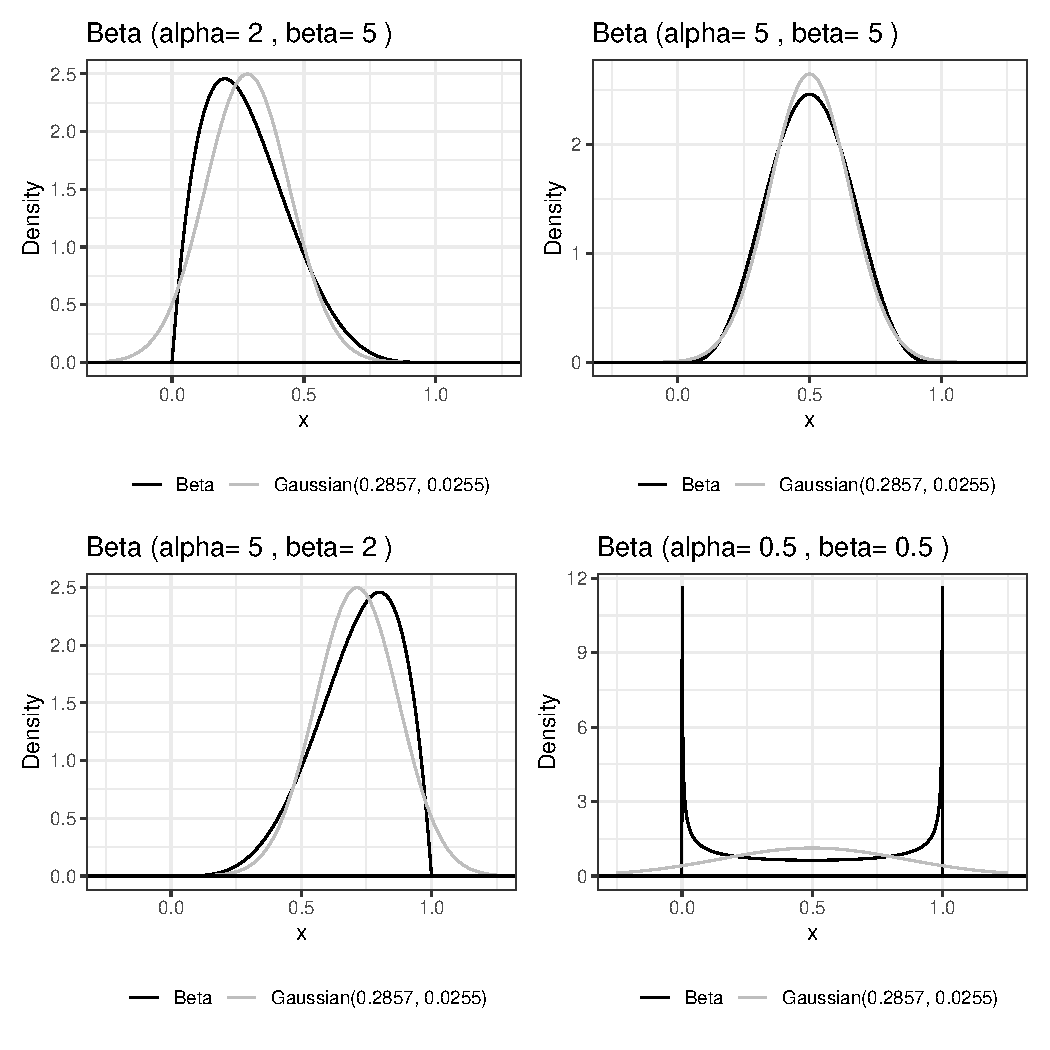
\includegraphics[width=\maxwidth]{figure/unnamed-chunk-1-1} 
\end{knitrout}


\section{Results}
Tie together the Introduction -- where you introduce the problem at hand -- and the methods --  what you propose to do to answer the question. Present your data, the results of your analyses, and how each reported aspect contributes to answering the question. This section should include table(s), statistic(s), and graphical displays. Make sure to put the results in a sensible order and that each result contributes a logical and developed solution. It should not just be a list. Avoid being repetitive. 

\subsection{Results Subsection}
Subsections can be helpful for the Results section, too. This can be particularly helpful if you have different questions to answer. 


\section{Discussion}
 You should objectively evaluate the evidence you found in the data. Do not embellish or wish-terpet (my made-up phase for making an interpretation you, or the researcher, wants to be true without the data \emph{actually} supporting it). Connect your findings to the existing information you provided in the Introduction.

Finally, provide some concluding remarks that tie together the entire paper. Think of the last part of the results as abstract-like. Tell the reader what they just consumed -- what's the takeaway message?

%%%%%%%%%%%%%%%%%%%%%%%%%%%%%%%%%%%%%%%%%%%%%%%%%%%%%%%%%%%%%%%%%%%%%%%%%%%%%%%%
% Bibliography
%%%%%%%%%%%%%%%%%%%%%%%%%%%%%%%%%%%%%%%%%%%%%%%%%%%%%%%%%%%%%%%%%%%%%%%%%%%%%%%%
\vspace{2em}

\noindent\textbf{Bibliography:} Note that when you add citations to your bib.bib file \emph{and}
you cite them in your document, the bibliography section will automatically populate here.

\begin{tiny}
\bibliography{bib}
\end{tiny}
\end{multicols}

%%%%%%%%%%%%%%%%%%%%%%%%%%%%%%%%%%%%%%%%%%%%%%%%%%%%%%%%%%%%%%%%%%%%%%%%%%%%%%%%
% Appendix
%%%%%%%%%%%%%%%%%%%%%%%%%%%%%%%%%%%%%%%%%%%%%%%%%%%%%%%%%%%%%%%%%%%%%%%%%%%%%%%%
\newpage
\onecolumn
\section{Appendix}

If you have anything extra, you can add it here in the appendix. This can include images or tables that don't work well in the two-page setup, code snippets you might want to share, etc.

\end{document}
